\chapter{Performance Analysis}
\label{chap:performance_analysis}

To determine the performance impact of \acp{iommu} on throughput and latency, we
conduct various measurements using the implementations described in
\Cref{chap:implementations}, i.e., \texttt{ixy.rs}, \texttt{ixgbevf} and
\texttt{iommu-leaks}.


\section{Methodology}
\label{sec:methodology}

% TODO: illustration of test setup?

\begin{table}
    \centering
    \begin{tabular}{lllrll}
        \textbf{CPU} & \textbf{Year} & \textbf{Arch.} & \textbf{Memory} & \textbf{NIC} & \textbf{NUMA} \\
        \toprule

        \multirow{2}{*}{Intel Xeon E3-1230v2} & \multirow{2}{*}{2012} &
        \multirow{2}{*}{Ivy Bridge} & \multirow{2}{*}{\SI{16}{\giga\byte}} & Intel X520-DA1 &
        \multirow{2}{*}{no} \\
        & & & & Intel X520-DA2 & \\ \hline

        \multirow{2}{*}{Intel Xeon E5-2620v3} & \multirow{2}{*}{2014} &
        \multirow{2}{*}{Haswell} & \multirow{2}{*}{\SI{32}{\giga\byte}} & Intel X520-DA2 &
        \multirow{2}{*}{no} \\
        & & & & Intel X540-T2 & \\ \hline

        \multirow{2}{*}{AMD EPYC 7551P} & \multirow{2}{*}{2017} &
        \multirow{2}{*}{Naples} & \multirow{2}{*}{\SI{128}{\giga\byte}} & Intel X550T &
        \multirow{2}{*}{yes} \\
        & & & & Intel X550T & \\

        \bottomrule
    \end{tabular}

    \caption{System configurations of servers used for performance analysis.}
    \label{tab:servers}
\end{table}

All measurements are performed on server pairs connected via two \SI{10}{\Gbps}
links. The devices under test use Intel \acp{nic} of the \texttt{ixgbe} family
that are compatible with our drivers, i.e., X520, X540 and X550. Each device
under test is equipped with two of these cards since two separate \acp{nic}
yield better performance than a dual-ported one (probably due to hardware
limitations of the \ac{nic} or the \ac{pcie} bus). \Cref{tab:servers} lists the
devices under test.

On the devices under test, we run the different implementations. For the
measurements, two applications are used on top of the drivers, a traffic
generator and a forwarder. The traffic generator allocates a memory pool and
repeatedly sends out the same buffers, only updating the sequence numbers of the
packets. The forwarder uses two devices, allocates a pool per device and
forwards packets bidirectionally, i.e., packets received by the first device are
sent out by the second and vice-versa. To simulate a somewhat realistic
workload, one byte of each packet is increased, enforcing the \ac{cpu} to load
the byte into the \ac{cpu} caches. On the second server, MoonGen
\cite{emmerich2015moongen} generates traffic with its
\texttt{l2-load-latency.lua} script.

All benchmarks are conducted at native \ac{cpu} frequency with dynamic
overclocking disabled. \ac{cpu} cores are pinned for the measurements. On NUMA
architectures, i.e., the AMD server, locality is obeyed for \ac{cpu} core
pinning and memory placement. \Cref{tab:cpus} contains details of the \acp{cpu}.
Two important characteristics emerge from the table: clockspeed has a huge
impact on single thread/core performance while the absolute number of cores is
crucial for overall \ac{cpu} performance.

Our benchmarking applications are executed on a single \ac{cpu} core in a single
thread as full support for multi-core systems is not implemented in the drivers
yet. On most systems this is not a limitation as hardware limits can be hit with
a single thread. It stands out from \Cref{tab:cpus} that -- although being the
oldest of the three \acp{cpu} -- the Intel Xeon E3 yields the highest per-thread
performance while the AMD \ac{cpu} performs worst. This observation is backed by
our baseline measurements (\Cref{sec:baseline_measurements}).

To reduce architecture-dependent overhead and assimilate the results of our
measurements, packet-prefetching is disabled in all implementations. If not
specified otherwise, packets are processed in batches of 32, ring sizes of 512
are used for RX and TX descriptors, and all \ac{dma}-able memory is allocated on
\SI{2}{\mebi\byte} huge pages. When the RX packet rate exceeds the host's packet
processing rate, i.e., the RX queue is full, packets are dropped by the
\ac{nic}.

Throughput and latency results of the implementations are measured on the second
server by MoonGen. Forwarded and generated packets contain \SI{60}{\byte} of
data, i.e., \SI{84}{\byte} with checksums and interpacket gap which is the
minimum Ethernet frame size, such that line rate at \SI{14.88}{\mega\pps} can be
achieved in all measurements.

\begin{table}
    \centering
    \begin{tabular}{llrrrr}
        \multirow{2}{*}{\textbf{CPU}} & \multirow{2}{*}{\textbf{Clock}} &
        \multirow{2}{*}{\textbf{Cores}} & \multirow{2}{*}{\textbf{L3-Cache}} &
        \multicolumn{2}{r}{\textbf{PassMark}} \\
        & & & & \textbf{ST} & \textbf{All} \\
        \toprule

        Intel Xeon E3-1230v2 & \SI{3.3}{\giga\Hz} &  4 &  \SI{8}{\mega\byte} & 1,996 &  6,192 \\
        Intel Xeon E5-2620v3 & \SI{2.4}{\giga\Hz} &  6 & \SI{15}{\mega\byte} & 1,700 &  7,979 \\
        AMD EPYC 7551P       & \SI{2.0}{\giga\Hz} & 32 & \SI{64}{\mega\byte} & 1,611 & 25,933 \\

        \bottomrule
    \end{tabular}

    \caption{\acsp{cpu} of devices under test and their PassMark scores for
    Single Thread (ST) and all cores.}
    \label{tab:cpus}
\end{table}

For measurements including an \ac{iommu}, pass-through mode is used for the
\ac{iommu} to reduce side effects from other \ac{io} devices on the host. All
measurements are conducted with Rust 1.50.0 on Debian Buster 10.6 with a Linux
4.19 kernel.


\section{Baseline Measurements}
\label{sec:baseline_measurements}

To determine the baseline performance of our devices under test, we run the
forwarder and the generator application in default configuration on all servers.
\Cref{fig:baseline-perf} shows the results. Since the generator application
generates traffic on a single port only, we run two instances on two different
devices for our measurements. Consequently, the bars on the left of
\Cref{fig:baseline-perf-throughput} show single core forwarding rate while the
bars on the right show dual core packet generation rate. Since the two instances
of the packet generator are executed independently of each other on two
different \ac{cpu} cores and devices, single core packet generation rate equals
(approximately) the measured results divided by two.

\begin{figure}%[!b]
	\centering
	\subfloat[Throughput]{%
        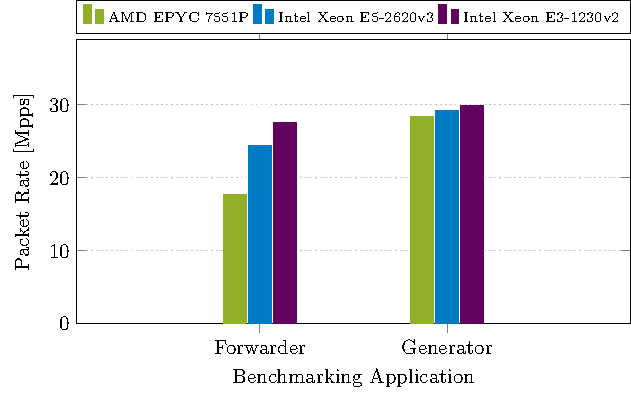
\includegraphics[width=0.46\textwidth]{figures/baseline-throughput}
		\label{fig:baseline-perf-throughput}
	}
	\subfloat[Latency]{%
        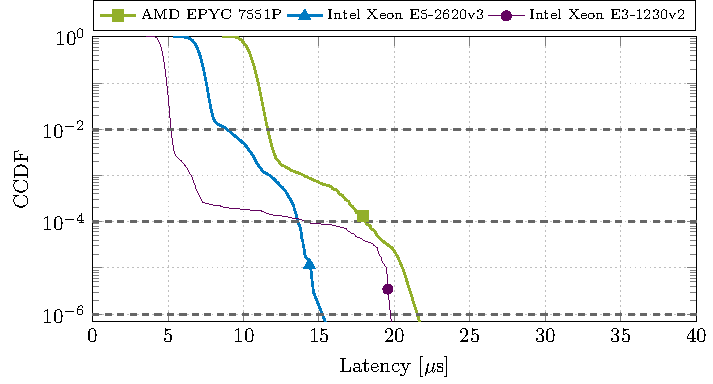
\includegraphics[width=0.54\textwidth]{figures/baseline-latency}
		\label{fig:baseline-perf-latency}
	}

    \caption{Baseline throughput and latency of servers used for performance
    measurements. Latency of forwarder measured with a total packet rate of
    \SI{10}{\mega\pps}.}
	\label{fig:baseline-perf}
\end{figure}

From \Cref{fig:baseline-perf-throughput}, it is particularly striking that the
packet forwarder on the AMD EPYC \ac{cpu} (packet rate: \SI{17.6}{\mega\pps}) is
about one third slower than on the Intel Xeon E5 \ac{cpu} (packet rate:
\SI{24.4}{\mega\pps}) although clockspeeds differ only by one sixth.

We use \ac{cpu} performance counters to profile the forwarder with both
\acp{cpu} and identify two reasons for the poor performance of the AMD \ac{cpu}:
the AMD \ac{cpu} executes about 1.75 instructions per cycle (IPC) while the
Intel \ac{cpu} runs about 2.1, and while 0.01-0.03\% of all branches are
mispredicted on the Intel \ac{cpu}, the AMD \ac{cpu} has a misprediction rate of
0.40\%.

Although AMD EPYC's Naples architecture is based on Zen, we find reports on poor
IPC counts and branch misses for the successor architecture of Zen -- Zen 2 --
which seem to support our findings \cite{lemire2019instructions,
lemire2019mispredictions}. Compared to Intel Skylake, the AMD Zen 2 \ac{cpu}
seems to take one to two additional cycles per branch misprediction.

Looking at \Cref{fig:baseline-perf-throughput}, both Intel \acp{cpu} stand out,
with the cheaper Xeon E3 \ac{cpu} introducing more variance into latency while
the more expensive Xeon E5 \ac{cpu} forwards traffic rather smoothly.


\section{Page Sizes}
\label{sec:page_sizes}

\begin{figure}[!b]
	\centering
	\subfloat[\SI{4}{\kibi\byte} pages, stack]{%
        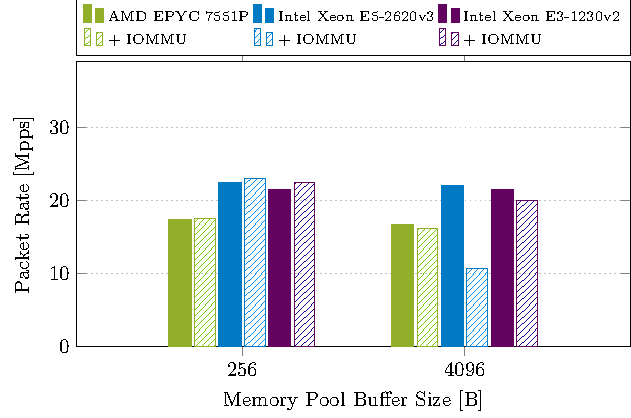
\includegraphics[width=0.46\textwidth]{figures/page-size-4k-throughput}
		\label{fig:page-size-4k-throughput}
	}
	\subfloat[\SI{4}{\kibi\byte} pages, queue]{%
        \includegraphics[width=0.46\textwidth]{figures/page-size-4k-queue-throughput}
		\label{fig:page-size-4k-queue-throughput}
	}
    \par
	\subfloat[\SI{2}{\mebi\byte} pages, stack]{%
        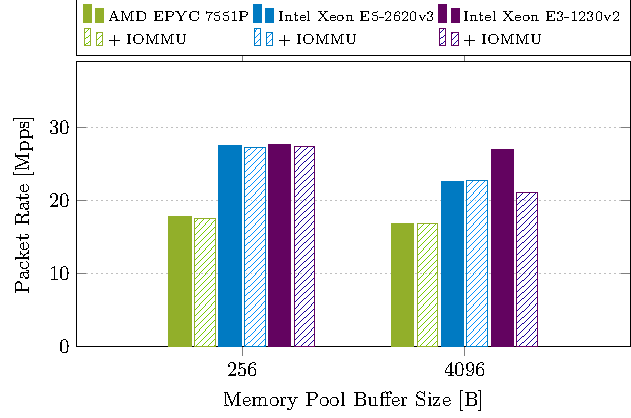
\includegraphics[width=0.46\textwidth]{figures/page-size-2m-throughput}
		\label{fig:page-size-2m-throughput}
	}
	\subfloat[\SI{2}{\mebi\byte} pages, queue]{%
        \includegraphics[width=0.46\textwidth]{figures/page-size-2m-queue-throughput}
		\label{fig:page-size-2m-queue-throughput}
	}
    \par
	\subfloat[\SI{1}{\gibi\byte} pages, stack]{%
        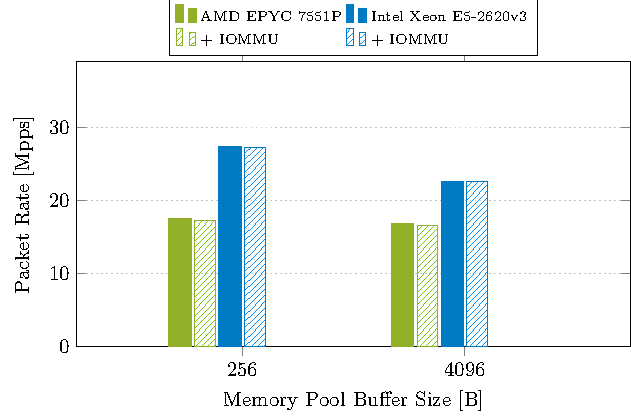
\includegraphics[width=0.46\textwidth]{figures/page-size-1g-throughput}
		\label{fig:page-size-1g-throughput}
	}
	\subfloat[\SI{1}{\gibi\byte} pages, queue]{%
        \includegraphics[width=0.46\textwidth]{figures/page-size-1g-queue-throughput}
		\label{fig:page-size-1g-queue-throughput}
	}

    \caption{Throughput of forwarder with different page sizes, memory pool
    buffer sizes and data structures for the memory pool.}
	\label{fig:page-size-throughput}
\end{figure}

It is well known that page sizes impact system performance. Page sizes are a
trade-off: When larger pages are used, overhead for page management decreases,
and page tables and the \ac{tlb} have to keep less entries. At the same time,
fragmentation and page swapping increases as even tiny amounts of data have to
be stored on whole pages and less pages can be kept in main memory at a time.
Smaller pages on the other hand increase page tables and put more pressure on
the \ac{tlb} since more pages have to be accessed for the same amount of data.
This can lead to \ac{tlb} thrashing: address translations are continuously
replaced by new translations in the \ac{tlb}, reducing effectiveness of the
cache. In extreme cases, addresses are re-translated for every page access,
i.e., the \ac{tlb} is practically no longer in use.

Available page sizes on a system depend on processor architecture and \ac{os}.
Linux on x86 uses \SI{4}{\kibi\byte} pages by default. With huge pages, sizes of
\SI{2}{\mebi\byte} or \SI{1}{\gibi\byte} can be used. These page sizes are also
supported by Intel's and AMD's \acp{iommu}.

To measure effects of different page sizes and number of pages, we run the
forwarder application with \SI{2}{\mebi\byte} and \SI{1}{\gibi\byte} huge pages
as well as our brute-force memory allocator to allocate memory on
\SI{4}{\kibi\byte} pages. \Cref{fig:page-size-throughput} visualizes packet
rates for different page sizes, memory pool buffer sizes and data structures for
the memory pool. For all measurements, RX and TX rings have a queue size of 256
descriptors. \Cref{fig:page-size-4k-throughput},
\Cref{fig:page-size-2m-throughput} and \Cref{fig:page-size-1g-throughput} use
the default implementation of the driver, i.e., a stack data structure for the
free buffers in the memory pool. There are no results for the Intel Xeon E3
\ac{cpu} and \SI{1}{\gibi\byte} pages since these page are not supported by the
\ac{cpu}.

We run our measurements with memory pool buffer sizes of \SI{256}{\byte} and
\SI{4,096}{\byte}. With \SI{4}{\kibi\byte} pages, different buffer sizes force
the driver to allocate varying numbers of \ac{dma}-able pages.

The exact number of allocated pages is determined by page size, buffer size and
number of descriptors. In case of huge pages, three huge pages are used per
device as all data structures fit onto single pages: one page is allocated for
the RX descriptor ring, one for the TX descriptor ring and one for the packet
memory pool. In case of \SI{4}{\kibi\byte} pages, 1~page is used for each
descriptor ring as each descriptor is \SI{16}{\byte} and thus 256~descriptors
fit onto a single page. The number of pages allocated for the memory pool
depends on the buffer size. Since \texttt{ixy.rs} allocates the memory pools by
default with twice as many buffers as RX/TX descriptors, the pool contains
512~packet buffers. With a buffer size of \SI{256}{\byte}, that totals to
\SI{128}{\kibi\byte}, i.e., 32~pages. With a buffer size of 4,096, 512~pages are
allocated. In summary, 34~pages are allocated per device with \SI{256}{\byte}
memory pool buffers and 514~pages are allocated with \SI{4,096}{\byte} buffers.

Various conclusions can be drawn from \Cref{fig:page-size-4k-throughput},
\Cref{fig:page-size-2m-throughput} and \Cref{fig:page-size-1g-throughput}. On
the AMD server, neither page size nor buffer size seem to have a significant
effect on throughput. The biggest performance drop happens with
\SI{4}{\kibi\byte} pages: Without \ac{iommu}, packet rate between
\SI{256}{\byte} memory pool buffers, i.e., 68 pages in total, and
\SI{4,096}{\byte} memory pool buffers, i.e., 1,028 pages, decreases by
\SI{0.7}{\mega\pps}. With \ac{iommu}, packet rate decreases twice as much, i.e.,
by \SI{1.4}{\mega\pps}.

On the Intel servers, results are inconsistent. The Xeon E5 \ac{cpu} exhibits
quite constant behavior with huge pages across all configurations: packet rates
drop with increasing buffer sizes, possibly due to decreased data locality.
Using \SI{4}{\kibi\byte} pages without \ac{iommu}, packet rate is almost
constant while with \ac{iommu} throughput goes down by more than 50\% when using
greater buffers, i.e., allocating more pages. We inspect this anomaly closer in
\Cref{fig:page-size-4k-omanyte}.

Like the AMD \ac{cpu}, the Intel Xeon E3 delivers constant throughput rates in
all non-\ac{iommu} configurations independent of page size and buffer size.
Compared to the Xeon E5 \ac{cpu}, \ac{iommu} performance seems abnormal for
\SI{4,096}{\byte} memory pool buffers with \SI{4}{\kibi\byte} and
\SI{2}{\mebi\byte} pages. For \SI{4}{\kibi\byte} pages, packet rate is
unexpectedly high while performance drops significantly for \SI{2}{\mebi\byte}
pages. The reasons for these unusual performance characteristics remain in the
dark. Notably, both Intel \acp{cpu} profit from huge pages unlike the AMD
\ac{cpu}.

In summary, our measurements imply that larger memory pool buffers and thus more
pages have a negative effect on packet throughput. In case of the \ac{iommu},
performance can degrade by more than 50\% on some \acp{cpu}. To back up our
results, we repeat the measurements and replace the free stack of the memory
pool by a queue. Our reasoning for changing the data structure is that with a
stack, the number of used pages by driver and device is not necessarily equal to
the number of allocated pages as there are probably some buffers at the bottom
of the stack that will never be used. With the stack, we know that the minimum
number of used pages is the number of pages used for buffers in the RX
descriptor ring + the number of pages used for buffers in the TX descriptor ring
+ the number of pages used for received and still-in-use packets.

In case of the 34~pages configuration, the minimum number of used pages is
2~pages for the RX/TX descriptor rings, 16~pages for the buffers in the RX
descriptor ring, 2~pages for a batch of 32 received packets, and 2~pages for a
batch of 32 packets in the transmit queue (as the transmit queue is cleaned
every 32 packets), i.e., 22~pages per device or 44~pages in total. In case of
the 514~pages configuration, we conclude with the same reasoning that a minimum
of 322~pages per device or 644~pages in total is used. We see from our
considerations that about two-thirds of the allocated pages have to be used by
driver and device.

By implementing the free stack of the memory pool as a queue, we enforce that
all allocated pages are used. \Cref{fig:page-size-4k-queue-throughput},
\Cref{fig:page-size-2m-queue-throughput} and
\Cref{fig:page-size-1g-queue-throughput} show the results of our measurements
using a queue for the free stack of the memory pool. Notably, there are only
minor differences in performance between the two data structures. It seems worth
mentioning that, in combination with the \acp{iommu}, there are four
configurations in which throughput with the queue is even slightly higher than
with the stack.

\begin{figure}%[!b]
	\centering
    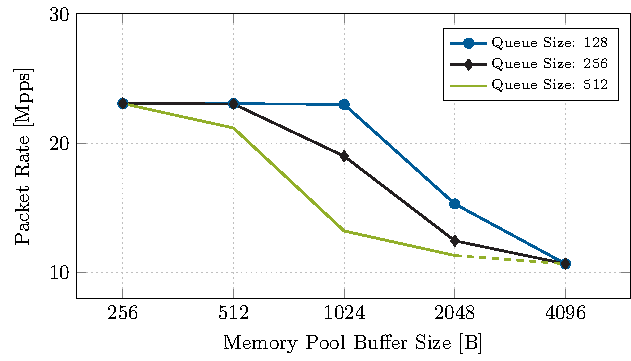
\includegraphics[width=0.46\textwidth]{figures/page-size-4k-omanyte-throughput}

    \caption{Throughput of forwarder on Intel Xeon E5-2620v3 with
    \SI{4}{\kibi\byte} pages, IOMMU enabled, and using a queue for the memory
    pool.}
	\label{fig:page-size-4k-omanyte}
\end{figure}

As noted before, \Cref{fig:page-size-4k-throughput} and
\Cref{fig:page-size-4k-queue-throughput} depict a drastical loss of performance
with \SI{4}{\kibi\byte} pages and larger memory pool buffer sizes on the Xeon E5
\ac{cpu} when using the \ac{iommu}. To determine whether this performance
degradation is caused by the number of used pages, we run the forwarder
application with different queue and memory pool buffer sizes on the Xeon E5
\ac{cpu}, using \SI{4}{\kibi\byte} pages, \ac{iommu} and a queue as data
structure for the memory pool. \Cref{fig:page-size-4k-omanyte} shows the
results of our measurements.

The stepwise decrease in packet rate for different queue and memory pool buffer
sizes seems to imply that the number of used pages is indeed the reason for loss
of throughput. With 2 + 64~pages per device, i.e., a queue size of 128 and
\SI{1,024}{\byte} buffers, a queue size of 256 and \SI{512}{\byte} buffers or a
queue size of 512 and \SI{256}{\byte} buffers, throughput is at its maximum.
With 2 + 128~pages, packet rate decreases between 1.9 and \SI{7.7}{\mega\pps}.
With 2 + 512~pages, throughput is at its worst with \SI{10.7}{\mega\pps}.

\begin{figure}%[!b]
	\centering
	\subfloat[Staggered in time]{%
        \includegraphics[width=0.46\textwidth]{figures/page-size-4k-omanyte-generator-one-throughput}
		\label{fig:page-size-4k-omanyte-generator-one-throughput}
	}
	\subfloat[Concurrently]{%
        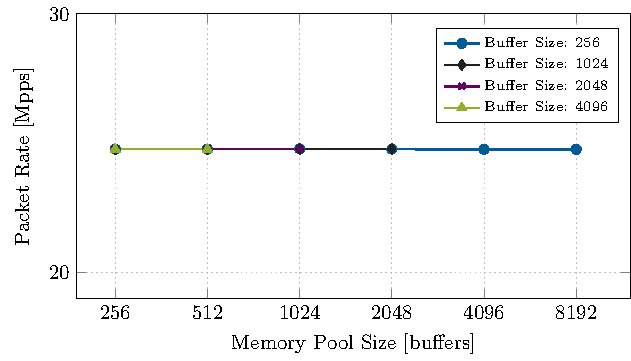
\includegraphics[width=0.46\textwidth]{figures/page-size-4k-omanyte-generator-two-throughput}
		\label{fig:page-size-4k-omanyte-generator-two-throughput}
	}
    \par
	\subfloat[Staggered in time with IOMMU]{%
        \includegraphics[width=0.46\textwidth]{figures/page-size-4k-omanyte-generator-iommu-one-throughput}
		\label{fig:page-size-4k-omanyte-generator-iommu-one-throughput}
	}
	\subfloat[Concurrently with IOMMU]{%
        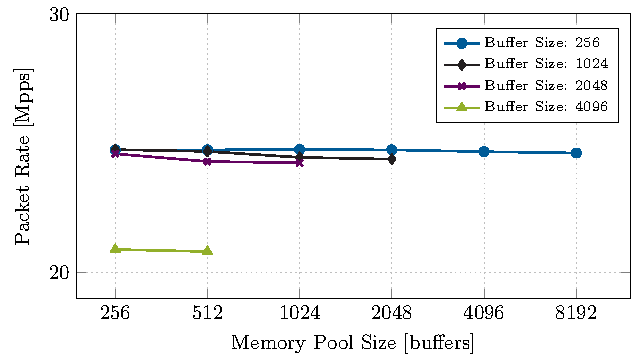
\includegraphics[width=0.46\textwidth]{figures/page-size-4k-omanyte-generator-iommu-two-throughput}
		\label{fig:page-size-4k-omanyte-generator-iommu-two-throughput}
	}

    \caption{Packet rate of two generator instances on Intel Xeon E5-2620v3 with
    \SI{4}{\kibi\byte} pages, different memory pool and buffer sizes.}
	\label{fig:page-size-generator}
\end{figure}

We repeat our measurements with the packet generator application on the Xeon E5
\ac{cpu}. \Cref{fig:page-size-generator} shows the results of our measurements.
We use a queue data structure for the memory pool and vary memory pool buffer
and memory pool size to run the generator with different numbers of
\SI{4}{\kibi\byte} pages, ranging from 16~pages (256~buffers with
\SI{256}{\byte} each) to 512~pages (8,192~buffers with \SI{256}{\byte} each, or
2,048~buffers with \SI{1,024}{\byte} each,~etc.). We run two instances of the
packet generator, each instance generating traffic on one device. We set the
queue size of RX and TX descriptor ring to 256 entries.
\Cref{fig:page-size-4k-omanyte-generator-one-throughput} and
\Cref{fig:page-size-4k-omanyte-generator-iommu-one-throughput} show the results
when running the generator instances staggered in time,
\Cref{fig:page-size-4k-omanyte-generator-two-throughput} and
\Cref{fig:page-size-4k-omanyte-generator-iommu-two-throughput} when running them
concurrently.

To our surprise, there seems to be no correlation between performance
degradation and the number of used pages. Packet rate in the non-\ac{iommu}
measurements is absolutely constant, with a loss of about 40k packets when
running both generators concurrently, while with \ac{iommu}, packet rate
decreases slightly with larger memory pool sizes, and significantly with a
buffer size of \SI{4,096}{\byte}. When running the two generators concurrently
with \SI{4,096}{\byte} buffers, packet rate goes down by \SI{3.7}{\mega\pps}
compared to \SI{256}{\byte} buffers using the same number of pages.

To verify whether packet rate in \Cref{fig:page-size-4k-omanyte} drops due to
only one \ac{iommu} domain being used for both devices, we modify the forwarder
of \Cref{fig:page-size-4k-omanyte} such that every device belongs to another
domain, and, since the devices can no longer access each other's \ac{dma}
memory, mirror packets received by the devices back onto the link. We check
packet rates in bullet point manner and note that there is almost no difference
in performance (\textasciitilde \SI{0.1}{\mega\pps}) when using one or two
domains for the devices. We also modify the packet generator
\Cref{fig:page-size-generator} to generate traffic on two devices, i.e., using
only one domain for both devices. Again, there is no noticeable performance
difference between one and two domains being used.

Our final guess as to why packet rate drops with the forwarder but not the
generator is that while both allocate 512~pages per device, the forwarder uses
both memory pools by each device: packets received by the first device end up in
a memory pool of the first device and are sent out from that pool by the second
device and vice versa. Thus, each device accesses more than 1,024~pages, twice
as many than with the generator. To confirm our suspicion, we modify the
generator such that every device sends out packets in an alternating manner from
two pools. Again, there is no noticeable drop of performance when increasing the
number of pages.

In summary, we note that on the AMD EPYC \ac{cpu}, there are no quantifiable
effects of the \ac{iommu} on performance. On the Intel \acp{cpu}, packet
throughput is impaired by the \ac{iommu} with a performance loss of more than
50\%. However, the reasons for this remain unclear: While our measurements in
\Cref{fig:page-size-4k-omanyte} imply a correlation between packet rate and the
numbers of pages in use, this is not confirmed by our packet generator.


\section{IOVA Address Widths}
\label{sec:iova_address_widths}

For \acp{iova}, any mappings can be chosen. Depending on page size and \ac{iova}
address widths, \acp{iommu} use different paging structures: To translate a
57-bit address to \SI{4}{\kibi\byte} pages, an Intel \ac{iommu} uses a 5-level
paging structure, for 48-bit and 39-bit addresses, 4 and 3 levels are used
respectively.

We run our packet forwarder application to determine the performance impact of
different \ac{iova} address widths. \Cref{fig:iova-address-widths-throughput}
shows the results of our measurements. We run the forwarder on two ports of a
single \ac{nic} (\Cref{fig:iova-address-widths-single-device-throughput}) and on
two distinct \acp{nic} (\Cref{fig:iova-address-widths-two-devices-throughput}).
There are no values for the Intel Xeon E-3 \ac{cpu} and 48-bit addresses as they
exceed the maximum \ac{iova} address widths of the Xeon's \ac{iommu} which is 39
bit.

When using a single dual-ported \ac{nic} for the forwarder, packet rate indeed
decreases by about \SI{1.7}{\mega\pps} on both Intel \acp{cpu} with 48-bit
addresses instead of 32-bit addresses. We repeat our measurements and note that
the loss of performance occurs as soon as \ac{iova} address widths surpass the
32-bit boundary.

When using two \acp{nic} for the forwarder, no significant change in performance
can be observed. Throughput increases slightly on the Intel \acp{cpu} by
\SI{0.3}{\mega\pps}.

We take a closer look at \Cref{fig:iova-address-widths-single-device-throughput}
with the different packet rates for different \ac{iova} address widths. We note
that 32~bit is not a boundary in the Intel \ac{iommu} paging structure. Compared
to \Cref{fig:iova-address-widths-two-devices-throughput}, throughput of the
forwarder is capped at a certain packet rate. We suspect that this is a
bottleneck at the \ac{pcie} level. A sufficient explanation is given by the
\ac{pcie} specification \cite{pcie2017specification}: The header of \ac{pcie}
memory read requests varies in size depending on the address widths, for 32-bit
addresses it is \SI{4}{\byte} smaller. Thus, more packets can be transmitted at
the \ac{pcie} level.

We conclude from these results that changes in performance with different
\ac{iova} address widths are not related to the \acp{iommu}.

\begin{figure}%[!b]
	\centering
	\subfloat[Throughput using 1 NIC]{%
        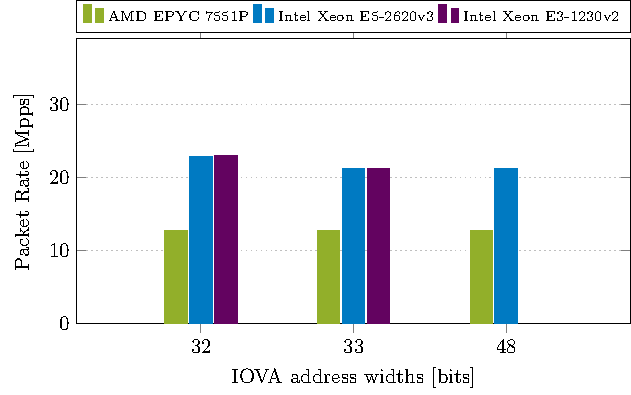
\includegraphics[width=0.46\textwidth]{figures/iova-address-widths-single-device-throughput}
		\label{fig:iova-address-widths-single-device-throughput}
	}
	\subfloat[Throughput using 2 NICs]{%
        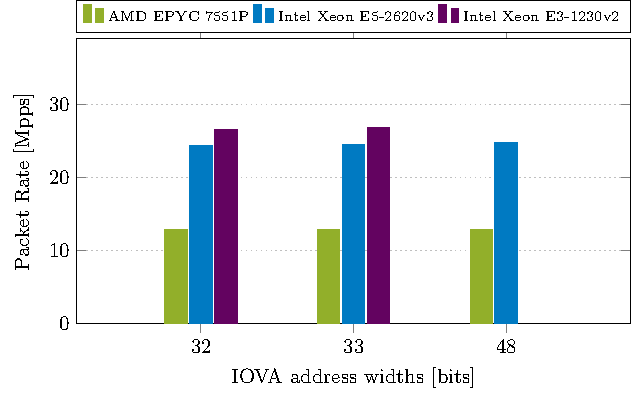
\includegraphics[width=0.46\textwidth]{figures/iova-address-widths-two-devices-throughput}
		\label{fig:iova-address-widths-two-devices-throughput}
	}

    \caption{Throughput of forwarder with 32, 33 and 48 bit wide IOVAs.}
	\label{fig:iova-address-widths-throughput}
\end{figure}


\section{Virtualization}
\label{sec:virtualization}

We take a look at \ac{iommu} impact on virtualization, i.e., \ac{sriov}. For
baseline measurements, we run the packet forwarder and packet generator
application on top of two \acp{vf}, with one \ac{vf} per device. We modify the
applications slightly to work with \ac{sriov}: instead of incrementing one byte
in the packets, the forwarder sets the source \ac{mac} address of each packet to
its own address -- otherwise, packets are dropped by the \ac{nic} due to its
anti-spoofing mechanism.

\Cref{fig:sriov-baseline} shows the results of our measurements. The AMD EPYC
\ac{cpu} is missing as only one of the two \ac{pcie} ports on the board supports
\ac{sriov}. Some values for the Intel Xeon E5 \ac{cpu} are also missing due to
\ac{iommu} group restrictions: On our server, \acp{vf} and \acp{pf} of the
\acp{nic} belong to the same \ac{iommu} group, making it impossible to access
them at the same time by multiple applications through \ac{vfio}, or through
\ac{vfio} and the native driver for the \ac{pf}.

As in our other measurements, two instances of the generator are run for the
measurements, one per device. Notably, compared to the unmodified forwarder in
\Cref{fig:baseline-perf-throughput}, the modified forwarder is about
\SI{6}{\mega\pps} slower on the Intel Xeon E5 \ac{cpu}, and about
\SI{2}{\mega\pps} slower on the Intel Xeon E3 \ac{cpu}.

The packet rates show that the \acp{iommu} have almost no impact on performance,
neither in the base configuration nor with \acp{vf}. Absurdly, packet rate with
\acp{vf} is \SI{5.3}{\mega\pps} greater on the Xeon E5 \ac{cpu} than without
\acp{vf}, and on the Xeon E3 \ac{cpu} the forwarder with \acp{vf} reaches a new
maximum of all measurements with \SI{27.6}{\mega\pps} (\SI{0.15}{\mega\pps}
faster compared to \Cref{fig:baseline-perf}).

\begin{figure}%[!b]
	\centering
	\subfloat[Throughput on Intel Xeon E5-2620v3]{%
        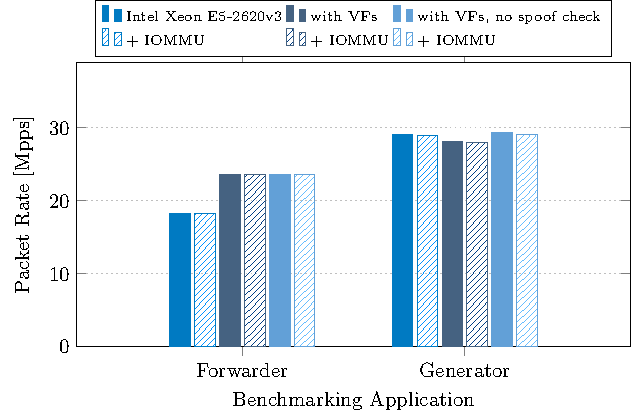
\includegraphics[width=0.49\textwidth]{figures/sriov-omanyte-throughput}
		\label{fig:sriov-omanyte-throughput}
	}
    \subfloat[Throughput on Intel Xeon E3-1230v2]{%
        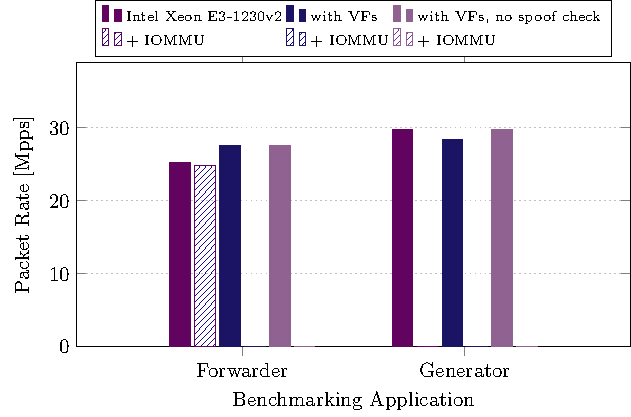
\includegraphics[width=0.49\textwidth]{figures/sriov-narva-throughput}
		\label{fig:sriov-narva-throughput}
	}
    \par
	\subfloat[Latency on Intel Xeon E5-2620v3]{%
        \includegraphics[width=0.49\textwidth]{figures/sriov-omanyte-latency}
		\label{fig:sriov-omanyte-latency}
	}
	\subfloat[Latency on Intel Xeon E3-1230v2]{%
        \includegraphics[width=0.49\textwidth]{figures/sriov-narva-latency}
		\label{fig:sriov-narva-latency}
	}

    \caption{Throughput and latency of modified forwarder with two devices, with
    and without VFs, with and without IOMMU. Latency of forwarder measured with
    a total packet rate of \SI{10}{\mega\pps}.}
	\label{fig:sriov-baseline}
\end{figure}

When running the generator application, we note that throughput is capped at
\SI{14.20}{\mega\pps} per port. We disable the \ac{mac} anti-spoofing mechanism
and reach line rate on the Xeon E3 \ac{cpu}, i.e., \SI{14.88}{\mega\pps} per
port. Thus, we put the cost of the spoof check at \SI{0.68}{\mega\pps} per port
or \SI{1.36}{\mega\pps} in total. We repeat this experiment on the AMD EPYC
\ac{cpu} and note that packet rate increases from \SI{14.08}{\mega\pps} to
\SI{14.35}{\mega\pps} when disabling the spoof check. To our surprise, on all
hosts the \ac{pf} driver of the Linux kernel reports some spoofed packets when
switching the spoof check on or off on the fly.

We also measure the latency. On the Xeon E3, latency of forwarder, and forwarder
with \acp{vf} resemble each other with, while latency of forwarder with
\ac{iommu} is on average \SI{1}{\micro\second} greater than without \ac{iommu}.
On the Xeon E5, latencies are also approximately the same, but tail latencies
diverge. Interestingly, forwarder and \ac{iommu} achieve the lowest tail
latencies, followed by the forwarder as-is, forwarder with \acp{vf} and
forwarder with \acp{vf} and \ac{iommu}.

We conclude that \acp{iommu} do not have a significant effect on throughput and
latency of \acp{vf}.


\section{Summary}
\label{sec:perf_summary}

Regarding the AMD EPYC \ac{cpu}, there are no measurable differences in
performance with AMD's \ac{iommu}. On Intel systems, \acp{iommu} have a negative
impact on performance in certain configurations. We suspect a correlation
between throughput and the amount of pages used by a device. To be more precise,
we assume that the \ac{iotlb} gets thrashed the more pages are used.

This assumption is not unreasonable: The datasheet for the Intel 82599 \acp{nic}
mentions changes in the \ac{pcie} transaction size to decrease the number of
\ac{pcie} transactions and thus thrashing of the \ac{iotlb}
\cite[p.~34]{intel2019datasheet}. And Neugebauer et al.
\cite{neugebauer2018understanding} report \ac{iotlb} thrashing on their Intel
Xeon E5-2630v4 based system, and determine an \ac{iotlb} size of 64 entries for
that particular \ac{iommu}. Unfortunately, our measurements confirm the
correlation between throughput and used pages only to some extent.

We were not able to identify any striking performance differences in relation to
\ac{iova} addresses or virtualization.

